\documentclass{article}

\usepackage{amsmath, amsthm, amssymb}
\usepackage{geometry}
\geometry{a4paper, top=25mm, left=10mm, right=10mm, bottom=30mm,
headsep=10mm, footskip=12mm}
\usepackage{graphicx}
\usepackage{lscape}
\begin{document} 

\begin{landscape}
\section{sextic BSplines}
\subsection{Functions}\begin{eqnarray*} \varphi_1 & = & \begin{array}{cc}
 \{ & 
\begin{array}{cc}
 91.54488033898493095698567221456806727274 x^6-274.6346410169547928709570166437042018182 x^5+320.4070811864472583494498527509882354546 x^4-183.0897606779698619139713444291361345455 x^3+45.77244016949246547849283610728403363637 x^2 & x\geq 0\land x<1 \\
 0 & \text{True}
\end{array}

\end{array}\\
\varphi_2 & = & \begin{array}{cc}
 \{ & 
\begin{array}{cc}
 -166.4932431061392953608767473533342364465 x^5+416.2331077653482384021918683833355911163 x^4-332.9864862122785907217534947066684728930 x^3+83.24662155306964768043837367666711822325 x^2 & x\geq 0\land x<1 \\
 0 & \text{True}
\end{array}

\end{array}\\
\varphi_3 & = & \begin{array}{cc}
 \{ & 
\begin{array}{cc}
 -885.6701049960537819172199376074271246735 x^6+2657.010314988161345751659812822281374021 x^5-2855.718351365481104515138644977793869941 x^4+1283.086177750693299444177601918452116514 x^3-198.7080363773197587634788321555124959203 x^2 & x\geq 0\land x<1 \\
 0 & \text{True}
\end{array}

\end{array}\\
\varphi_4 & = & \begin{array}{cc}
 \{ & 
\begin{array}{cc}
 38764.45509995756892370496117521182922496 x^6-59248.09483310993266995983480844125712847 x^5+33679.00741002346761775787255220369070116 x^4-8393.340079305285660767519172781372390886 x^3+761.9975491090004465558888089263127665824 x^2 & x\geq 0\land x<\frac{1}{2} \\
 -3802.509033523003109102383938420657916763 x^6+20765.58697814694982695539745388520273068 x^5-46527.58188362280979526416528171180936058 x^4+54649.79319666166073587879845563577516304 x^3-35411.90519305723433818995451036242896472 x^2+11971.87764102399516963749114176270372982 x-1645.261705629558489915183320788785381476 & x\geq \frac{1}{2}\land x<1
\end{array}

\end{array}\\
\varphi_5 & = & \begin{array}{cc}
 \{ & 
\begin{array}{cc}
 108941.8618503386885868446516297774742574 x^6-151596.3728091002308217330842861311546587 x^5+74934.95216280847198610842741116501212336 x^4-15341.84347240420315088307822228626939713 x^3+1071.281044938382112888434276693720087993 x^2 & x\geq 0\land x<\frac{1}{2} \\
 -30765.96023973972291507649880211383574873 x^6+143283.8452030568545293816868324778843140 x^5-274930.8162684264245093177017703529510883 x^4+278118.0779656846079755260147079969438909 x^3-156408.8060952738960459382072934400220722 x^2+46363.17879035373104611973619459460974719 x-5659.519355655150080695029869162629042874 & x\geq \frac{1}{2}\land x<1
\end{array}

\end{array}\\
\varphi_6 & = & \begin{array}{cc}
 \{ & 
\begin{array}{cc}
 17131.76102426852674168795377419958344117 x^6-24503.42685482673860549648520631033211477 x^5+12465.85167926065233224200524235515599878 x^4-2591.765513830143595241135199592148161804 x^3+174.8896003876931644400279976224297356710 x^2 & x\geq 0\land x<\frac{1}{2} \\
 24012.58101317181558567361780371120694192 x^6-99450.05476040147967605542291876226767051 x^5+166700.1631506331933221190414066604050792 x^4-144287.2953980828935819913342972583712964 x^3+67775.97256422868723786672976835031727234 x^2-16315.92381376496215200021450002304427112 x+1564.557244215639264387582737321753944614 & x\geq \frac{1}{2}\land x<1
\end{array}

\end{array}\\
\varphi_7 & = & \begin{array}{cc}
 \{ & 
\begin{array}{cc}
 -46652.12713008827968561829185969001149456 x^6+68938.67771281340700903785691848857447309 x^5-37832.76300574257584767258647760391271437 x^4+9303.411477530918170349996676772490368245 x^3-906.0132094952703555270700595442025532034 x^2+3.148430272070665959998628308697916830028 & x\geq 0\land x<\frac{1}{2} \\
 9623.230458592658705877988655890326301799 x^6-46795.56896293698261935916776062843546198 x^5+93840.10715166215880325259180454251748625 x^4-99243.27759927974100127085941772573149341 x^3+58324.97519661487114413561741699834302374 x^2-18042.08413891019363594111693118934201311 x+2292.617894257228603304946232112322156724 & x\geq \frac{1}{2}\land x<1 \\
 2974.776866053316170095658616680461201333 x^6+13957.25144373940189971471121014813726796 x^5+26907.36480577790545089981637926837109578 x^4+27246.55761925484326914685881552487422354 x^3+15263.11918442669709216705937437819478466 x^2+4478.428711823373702493203468597332150010 x+536.9769185597001581922391239433165597385 & x\geq -1\land x<-\frac{1}{2} \\
 -17648.80800198385665613192806615975415404 x^6-31650.40518109180981423418773612429375837 x^5-21203.92572561843772789546379480141055044 x^4-6343.241912228100471557506434496122144120 x^3-737.4844428134965821481363623775881345822 x^2+3.148430272070665959998628308697916830028 & x\geq -\frac{1}{2}\land x<0
\end{array}

\end{array}\\
\varphi_8 & = & \begin{array}{cc}
 \{ & 
\begin{array}{cc}
 76036.15157894178788415122761236902096279 x^6-116363.6865015044629568216774153943493864 x^5+68252.42794704896771064863620083162408739 x^4-19192.72589164746582439724546564244590910 x^3+2592.802786801108943316161494368065641688 x^2-134.8124572549120871261097864239869057244 x+0.1931169449885436438460283441475338336181 & x\geq 0\land x<\frac{1}{2} \\
 -16677.19071911319483649668014663196196827 x^6+81078.86357140057394278142387704851674897 x^5-162542.5179050875086606009690955064635327 x^4+171839.9219144162742582703256942526720652 x^3-100944.7998493916040361438287432990466977 x^2+31208.73203356071924495351828041511939523 x-3963.009045785259912763789866278836010765 & x\geq \frac{1}{2}\land x<1 \\
 4316.603712205862860456844482315424192144 x^6+20259.40037215316116469980446590482658774 x^5+39071.64942278307812484628857859156154394 x^4+39581.96260125513082081041675697018313440 x^3+22185.19988176121468543168302843658264015 x^2+6513.730063358720747059314664697274267036 x+781.6400200168570618347197982287156129370 & x\geq -1\land x<-\frac{1}{2} \\
 -39600.02798752129631122634913056576033049 x^6-72571.99211266711058592327071320164868881 x^5-50828.83394822783917213571440710161849844 x^4-16744.31188930879729473359413716568813728 x^3-2533.248529077398164299860291495543391103 x^2-134.8124572549120871261097864239869057244 x+0.1931169449885436438460283441475338336181 & x\geq -\frac{1}{2}\land x<0
\end{array}

\end{array}\end{eqnarray*}
\end{landscape}
\begin{landscape}
\subsection{Graphics}
\begin{tabular}{cccc}
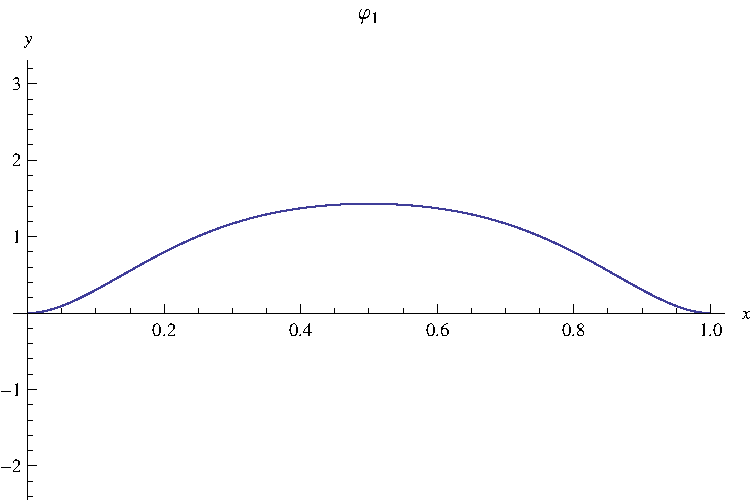
\includegraphics[width=5.0cm]{sextic_bspline_1.pdf}& 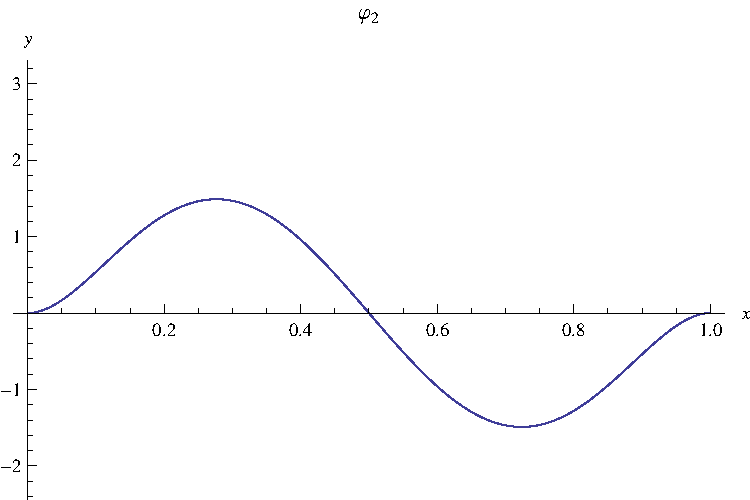
\includegraphics[width=5.0cm]{sextic_bspline_2.pdf}& 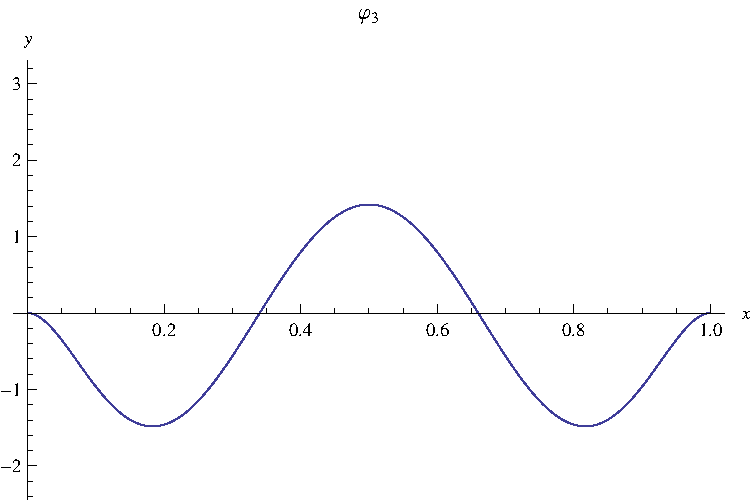
\includegraphics[width=5.0cm]{sextic_bspline_3.pdf}& 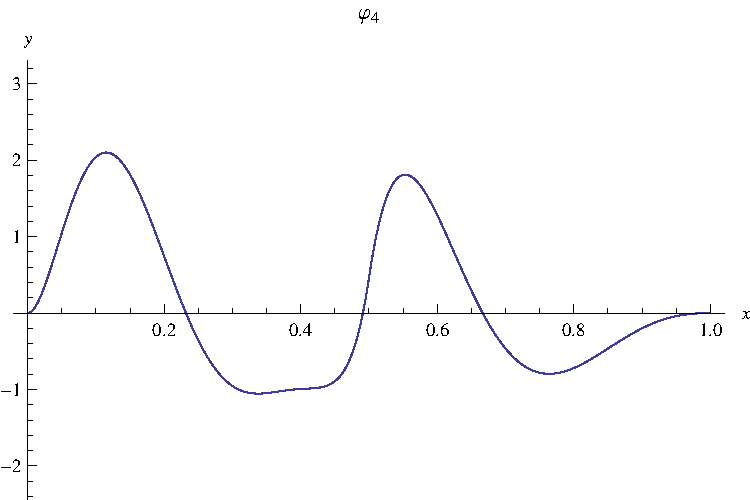
\includegraphics[width=5.0cm]{sextic_bspline_4.pdf} \\
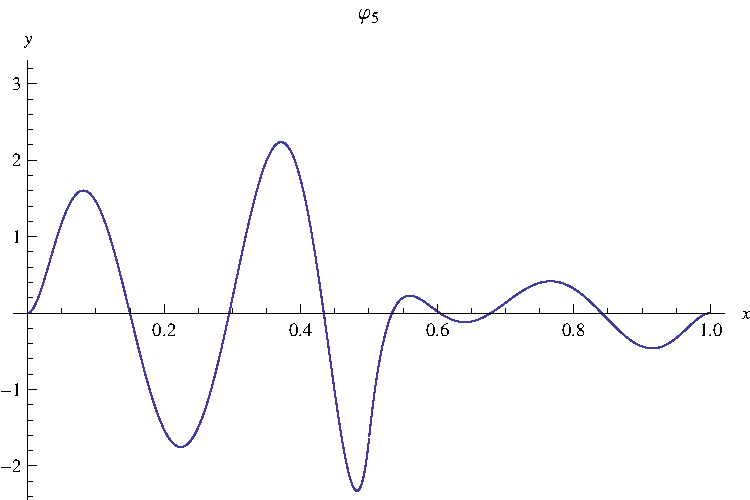
\includegraphics[width=5.0cm]{sextic_bspline_5.pdf}& 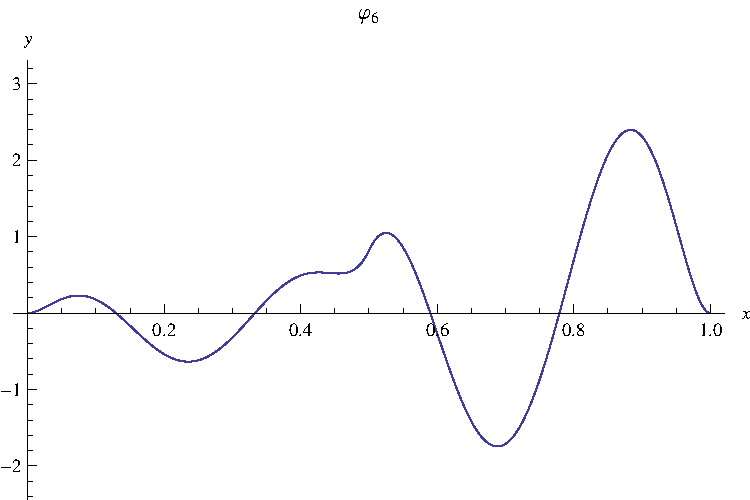
\includegraphics[width=5.0cm]{sextic_bspline_6.pdf}& 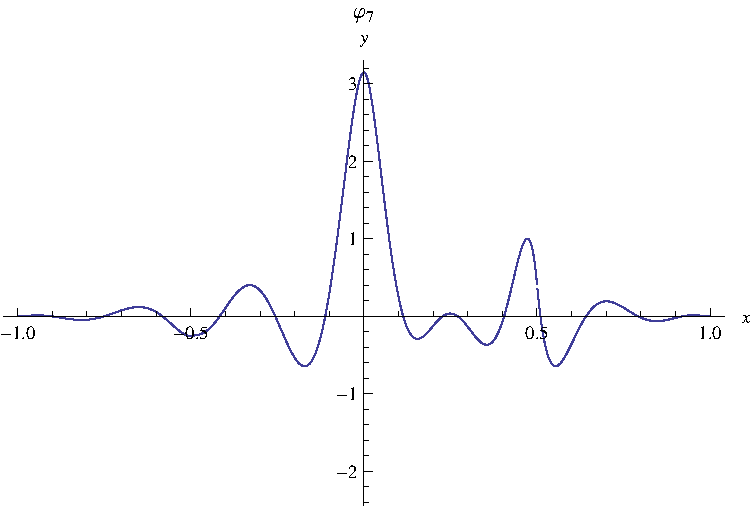
\includegraphics[width=5.0cm]{sextic_bspline_7.pdf}& 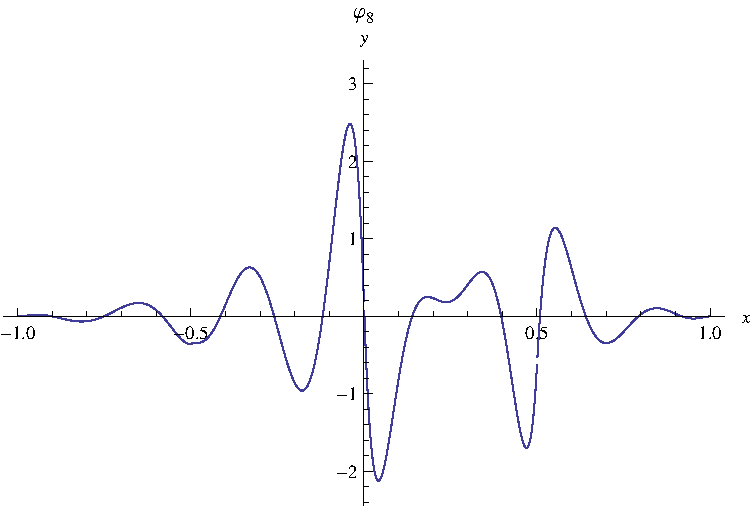
\includegraphics[width=5.0cm]{sextic_bspline_8.pdf} \\
\end{tabular} 
 \end{landscape}
 \begin{landscape}
 \subsection{Validation}$$ \begin{array}{l|llllllll}
\int_{-1}^1 f_1(x)f_2(x) dx& \varphi_1(x)& \varphi_2(x)& \varphi_3(x)& \varphi_4(x)& \varphi_5(x)& \varphi_6(x)& \varphi_7(x)& \varphi_8(x) \\ \hline 
 \varphi_1(x) & 1.0000 & 0 & 0 & 0.\cdot 10^{(-883)} & 0.\cdot 10^{(-881)} & 0.\cdot 10^{(-882)} & 0.\cdot 10^{(-746)} & 0.\cdot 10^{(-723)} \\ 
\varphi_2(x) & 0 & 1.0000 & 0 & 0.\cdot 10^{(-882)} & 0.\cdot 10^{(-881)} & 0.\cdot 10^{(-882)} & 0.\cdot 10^{(-746)} & 0.\cdot 10^{(-723)} \\ 
\varphi_3(x) & 0 & 0 & 1.0000 & 0.\cdot 10^{(-882)} & 0.\cdot 10^{(-880)} & 0.\cdot 10^{(-881)} & 0.\cdot 10^{(-745)} & 0.\cdot 10^{(-722)} \\ 
\varphi_4(x) & 0.\cdot 10^{(-883)} & 0.\cdot 10^{(-882)} & 0.\cdot 10^{(-882)} & 1.0000 & 0.\cdot 10^{(-878)} & 0.\cdot 10^{(-879)} & 0.\cdot 10^{(-744)} & 0.\cdot 10^{(-721)} \\ 
\varphi_5(x) & 0.\cdot 10^{(-881)} & 0.\cdot 10^{(-881)} & 0.\cdot 10^{(-880)} & 0.\cdot 10^{(-878)} & 1.0000 & 0.\cdot 10^{(-878)} & 0.\cdot 10^{(-743)} & 0.\cdot 10^{(-720)} \\ 
\varphi_6(x) & 0.\cdot 10^{(-882)} & 0.\cdot 10^{(-882)} & 0.\cdot 10^{(-881)} & 0.\cdot 10^{(-879)} & 0.\cdot 10^{(-878)} & 1.0000 & 0.\cdot 10^{(-743)} & 0.\cdot 10^{(-720)} \\ 
\varphi_7(x) & 0.\cdot 10^{(-746)} & 0.\cdot 10^{(-746)} & 0.\cdot 10^{(-745)} & 0.\cdot 10^{(-744)} & 0.\cdot 10^{(-743)} & 0.\cdot 10^{(-743)} & 1.0000 & 0.\cdot 10^{(-720)} \\ 
\varphi_8(x) & 0.\cdot 10^{(-723)} & 0.\cdot 10^{(-723)} & 0.\cdot 10^{(-722)} & 0.\cdot 10^{(-721)} & 0.\cdot 10^{(-720)} & 0.\cdot 10^{(-720)} & 0.\cdot 10^{(-720)} & 1.0000 \\ 
\end{array} $$
$$ \begin{array}{l|llllllll}
\int_{-1}^1 f_1(x)f_2(x-1) dx& \varphi_1(x-1)& \varphi_2(x-1)& \varphi_3(x-1)& \varphi_4(x-1)& \varphi_5(x-1)& \varphi_6(x-1)& \varphi_7(x-1)& \varphi_8(x-1) \\ \hline 
 \varphi_1(x) & 0 & 0 & 0 & 0 & 0 & 0 & 0.\cdot 10^{(-745)} & 0.\cdot 10^{(-722)} \\ 
\varphi_2(x) & 0 & 0 & 0 & 0 & 0 & 0 & 0.\cdot 10^{(-745)} & 0.\cdot 10^{(-722)} \\ 
\varphi_3(x) & 0 & 0 & 0 & 0 & 0 & 0 & 0.\cdot 10^{(-744)} & 0.\cdot 10^{(-721)} \\ 
\varphi_4(x) & 0 & 0 & 0 & 0 & 0 & 0 & 0.\cdot 10^{(-743)} & 0.\cdot 10^{(-720)} \\ 
\varphi_5(x) & 0 & 0 & 0 & 0 & 0 & 0 & 0.\cdot 10^{(-742)} & 0.\cdot 10^{(-719)} \\ 
\varphi_6(x) & 0 & 0 & 0 & 0 & 0 & 0 & 0.\cdot 10^{(-742)} & 0.\cdot 10^{(-719)} \\ 
\varphi_7(x) & 0 & 0 & 0 & 0 & 0 & 0 & -4.14899\cdot 10^{(-463)} & -1.12244\cdot 10^{(-462)} \\ 
\varphi_8(x) & 0 & 0 & 0 & 0 & 0 & 0 & 9.19398\cdot 10^{(-463)} & 1.91293\cdot 10^{(-462)} \\ 
\end{array} $$ 
\end{landscape} 
 \begin{landscape}
 \subsection{sextic BSpline dirichlet boundary Functions}
 \begin{eqnarray*}
 \varphi_{\text{left},1} & = & \begin{array}{cc}
 \{ & 
\begin{array}{cc}
 102649.1862935818098471621204534681840656 x^6-156895.5266375797874984674699770156543542 x^5+91818.42648538611844540964455045045118192 x^4-25712.97828289558209674326744593943264030 x^3+3445.647413608603430975125157850890442093 x^2-175.3966580264086972945724661761787184603 x & x\geq 0\land x<\frac{1}{2} \\
 -22465.68399455391676651199428939944933501 x^6+109221.4130245024199979106506305701297231 x^5-218963.3233773576215812994474486816511123 x^4+231490.8233242187503121428259088997096494 x^3-135987.9066346574383395282378479550069963 x^2+42043.67565090051267734450034748353688826 x-5338.997993052706300058297300917268817113 & x\geq \frac{1}{2}\land x<1
\end{array}

\end{array}\\ 
\varphi_{\text{right},1} & = & \begin{array}{cc}
 \{ & 
\begin{array}{cc}
 6432.996235116041790780994973451490347364 x^6-8405.146554366369778794290647159025667371 x^5+3760.713099610489913319052425315307555985 x^4-659.6805517558841401021923283720511284328 x^3+36.15011052579801880419199462033276154860 x^2 & x\geq 0\land x<\frac{1}{2} \\
 -59935.80217187449960092705830345873556999 x^6+249708.8111977501583239188806681684763598 x^5-426576.2810673392200771194167350430915021 x^4+382483.2166680030314255958657332511516383 x^3-189914.5580958755464807750265848863925963 x^2+49545.57027883132429937230356684934578785 x-5310.956809495247890065548344880754117566 & x\geq \frac{1}{2}\land x<1
\end{array}

\end{array}\end{eqnarray*}
\end{landscape}
\begin{landscape}
\subsection{BSpline Dirichlet boundary Graphics}
\begin{tabular}{c}
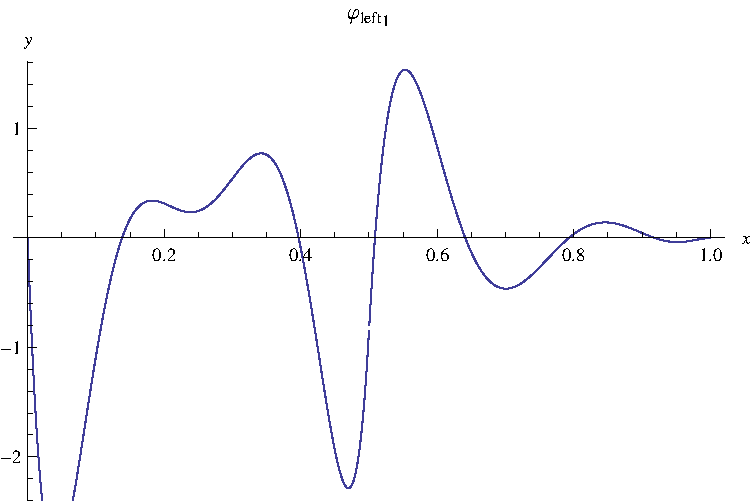
\includegraphics[width=20.cm]{sextic_bspline_dleft_1.pdf}\end{tabular} 
 \\ 
\begin{tabular}{c}
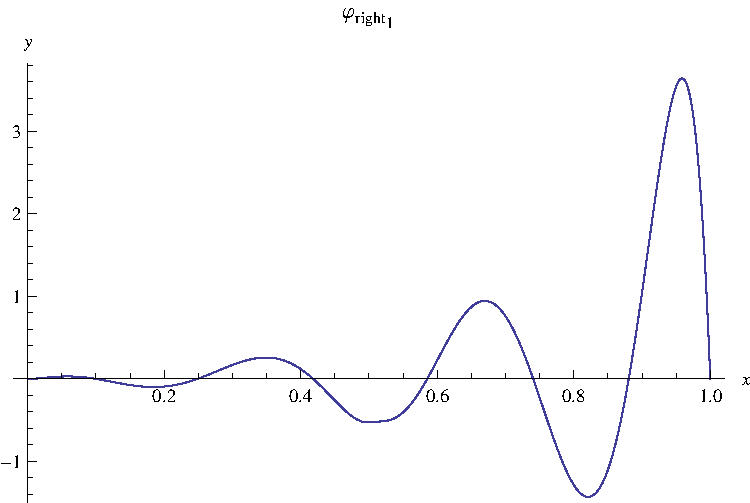
\includegraphics[width=20.cm]{sextic_bspline_dright_1.pdf}\end{tabular} 
 \end{landscape}
 \begin{landscape}
 \subsection{Validation}$$ \begin{array}{l|l}
\int_{-1}^1 f_1(x)f_2(x) dx& \varphi_{\text{left},1}(x) \\ \hline 
 \varphi_{\text{left},1}(x) & 1.0000 \\ 
\end{array} $$
$$ \begin{array}{l|llllllll}
\int_{-1}^1 f_1(x)f_2(x) dx& \varphi_1(x)& \varphi_2(x)& \varphi_3(x)& \varphi_4(x)& \varphi_5(x)& \varphi_6(x)& \varphi_7(x)& \varphi_8(x) \\ \hline 
 \varphi_{\text{left},1}(x) & 0.\cdot 10^{(-712)} & 0.\cdot 10^{(-712)} & 0.\cdot 10^{(-711)} & 0.\cdot 10^{(-709)} & 0.\cdot 10^{(-709)} & 0.\cdot 10^{(-709)} & -0.59390 & 0.73219 \\ 
\end{array} $$ 
$$ \begin{array}{l|llllllll}
\int_{-1}^1 f_1(x)f_2(x) dx& \varphi_1(x-1)& \varphi_2(x-1)& \varphi_3(x-1)& \varphi_4(x-1)& \varphi_5(x-1)& \varphi_6(x-1)& \varphi_7(x-1)& \varphi_8(x-1) \\ \hline 
 \varphi_{\text{left},1}(x) & 0 & 0 & 0 & 0 & 0 & 0 & 1.22929\cdot 10^{(-462)} & 2.57838\cdot 10^{(-462)} \\ 
\end{array} $$ 
$$ \begin{array}{l|l}
\int_{-1}^1 f_1(x)f_2(x) dx& \varphi_{\text{right},1}(x) \\ \hline 
 \varphi_{\text{right},1}(x) & 1.0000 \\ 
\end{array} $$
$$ \begin{array}{l|llllllll}
\int_{-1}^1 f_1(x)f_2(x) dx& \varphi_1(x)& \varphi_2(x)& \varphi_3(x)& \varphi_4(x)& \varphi_5(x)& \varphi_6(x)& \varphi_7(x)& \varphi_8(x) \\ \hline 
 \varphi_{\text{right},1}(x) & 0.\cdot 10^{(-704)} & 0.\cdot 10^{(-703)} & 0.\cdot 10^{(-703)} & 0.\cdot 10^{(-701)} & 0.\cdot 10^{(-700)} & 0.\cdot 10^{(-701)} & -1.707\cdot 10^{(-462)} & 2.8889\cdot 10^{(-462)} \\ 
\end{array} $$ 
$$ \begin{array}{l|llllllll}
\int_{-1}^1 f_1(x)f_2(x) dx& \varphi_1(x-1)& \varphi_2(x-1)& \varphi_3(x-1)& \varphi_4(x-1)& \varphi_5(x-1)& \varphi_6(x-1)& \varphi_7(x-1)& \varphi_8(x-1) \\ \hline 
 \varphi_{\text{right},1}(x) & 0 & 0 & 0 & 0 & 0 & 0 & 0.61486 & 0.68036 \\ 
\end{array} $$ 
$$ \begin{array}{l|l}
\int_{-1}^1 f_1(x)f_2(x) dx& \varphi_{\text{left},1}(x) \\ \hline 
 \varphi_{\text{right},1}(x) & 3.8948\cdot 10^{(-462)} \\ 
\end{array} $$ 
\end{landscape} 
 \begin{landscape}
\section{Wavelets}
\subsection{Functions}
 \begin{eqnarray*}
\Psi_1 & = & \begin{array}{cc}
 \{ & 
\begin{array}{cc}
 -962771.1106459966674395452820381064572263 x^6+638138.1555384813615842604853672795985323 x^5-145464.7516174103668765169811204034838569 x^4+13015.03646934811473724484319484262627291 x^3-361.3823228396999880352252284658308163075 x^2 & x\geq 0\land x<\frac{1}{4} \\
 -75976.13811463592923941583657377023455165 x^6+59483.36422028166931862259884797423867420 x^5+32103.92807012353775964798520508691296290 x^4-50664.71101300210780202902555715650657258 x^3+21341.93501728655425816448961913190667223 x^2-3903.961396835683522574460926579593381982 x+269.4913056393380467007888738685220204678 & x\geq \frac{1}{4}\land x<\frac{1}{2} \\
 -480978.8515436724449992156356310085499130 x^6+1.439021467864795743320977518919924301490\times 10^6 x^5-1.624167064915820345331540735852922142531\times 10^6 x^4+796876.2168252809862981617739372448776552 x^3-100813.4064632122068167565007894677070349 x^2-44436.46792304360289797565980902870059820 x+11866.50267914172467998036165458928120980 & x\geq \frac{1}{2}\land x<\frac{3}{4} \\
 -61778.90532265949604168418792530617293368 x^6+337994.6996191994424136233352848022231027 x^5-771188.0187275259402450871755274629980220 x^4+939246.8800353236336062830457285299789012 x^3-643939.0003028540136449430225426636100304 x^2+235589.3692498006516333740611374151975335 x-35925.02455128427772156605615531461855145 & x\geq \frac{3}{4}\land x<1
\end{array}

\end{array}\\
\Psi_2 & = & \begin{array}{cc}
 \{ & 
\begin{array}{cc}
 5.327930976124082588470701771807200086723\times 10^6 x^6-3.604555401926520097380394752909744282401\times 10^6 x^5+849004.5644483800146879880479297767616816 x^4-79974.62372973319376840234990896647841058 x^3+2409.100136945362985961836385818343626504 x^2 & x\geq 0\land x<\frac{1}{4} \\
 -419473.3110045658775384761752700188054884 x^6+1.235962011388154460246569563547068652870\times 10^6 x^5-1.418004609824251610695330596400865009314\times 10^6 x^4+823923.4199384155802333555365321264939179 x^3-258101.3347994526278818495541428484674089 x^2+41597.24893855276404690438705515203569786 x-2709.205308078518070397573757526048747929 & x\geq \frac{1}{4}\land x<\frac{1}{2} \\
 -35795.97221339468560695229977226951638802 x^6+114112.3149063878946251068205883113524481 x^5-144896.9186204638023456851673343939458918 x^4+92159.97008536248857606375234180015965186 x^3-29937.75748891100833224180498549865061643 x^2+4340.942543114512334989142026095102569487 x-157.9013101567433647926046623898530664804 & x\geq \frac{1}{2}\land x<\frac{3}{4} \\
 -4984.172574122915490975588942556005328791 x^6+26194.69144916443104170322520761853933420 x^5-57480.14907280855437909436346029976604125 x^4+67447.27237896128426649744264155750150348 x^3-44657.09710233331104738876725195256614793 x^2+15824.55155793232454900006803767502725215 x-2345.096636793258939742016232042730571862 & x\geq \frac{3}{4}\land x<1
\end{array}

\end{array}\\
\Psi_3 & = & \begin{array}{cc}
 \{ & 
\begin{array}{cc}
 -1.955649100405725757194484719045476044743\times 10^6 x^6+1.289515975177136994169235167488488312522\times 10^6 x^5-292518.7113910198875854690876234882048429 x^4+26156.49183603082795735820762506298483382 x^3-735.2695019565960282131233024267695795030 x^2 & x\geq 0\land x<\frac{1}{4} \\
 4.764941530884936772380347862200071526608\times 10^6 x^6-1.010250064937683272587127476248585223130\times 10^7 x^5+8.768846278567381895022906366527797237535\times 10^6 x^4-3.987816278918117385782500504633330676215\times 10^6 x^3+1.002442535613118728481462546114903991921\times 10^6 x^2-132182.4559454339882563241171305962010068 x+7153.615755498387306690205573159735527272 & x\geq \frac{1}{4}\land x<\frac{1}{2} \\
 178991.8160899043676647269099000420831393 x^6-490675.2747935236643356051491411494279736 x^5+451668.8577405695487752272485076745837181 x^4-89055.62025482538588898668937226642703647 x^3-102917.0014214939271047406406487510024109 x^2+63865.43947190033468786544158335782795976 x-10766.01988780736546437115716161289820653 & x\geq \frac{1}{2}\land x<\frac{3}{4} \\
 16459.01403836627430186985323025949733103 x^6-99255.84977532291023503607721755824450810 x^5+246395.3025770860066995650470601921059423 x^4-322755.1406377640633344023425291958153086 x^3+235542.7227338118080361779054466809871390 x^2-90876.06921625854750344770484030871356696 x+14490.02028008143203527331884993018297137 & x\geq \frac{3}{4}\land x<1
\end{array}

\end{array}\\
\Psi_4 & = & \begin{array}{cc}
 \{ & 
\begin{array}{cc}
 1.325679596774854635759826858283359200143\times 10^7 x^6-4.939216603001270834781222261186118377904\times 10^7 x^5+7.633716678426424192966357240768195131366\times 10^7 x^4-6.264208510195438680258859927971423364106\times 10^7 x^3+2.878464780194387915347605794714700478831\times 10^7 x^2-7.022471396671596322701069519074135187304\times 10^6 x+710627.9039722839130652409911853917871200 & x\geq \frac{1}{2}\land x<\frac{3}{4} \\
 -2.774465094435150826503717041237412143174\times 10^6 x^6+1.503177445874082317591728642542605340873\times 10^7 x^5-3.386306953734642082480569415229564226902\times 10^7 x^4+4.059880950400652581183763763990848462129\times 10^7 x^3-2.731938963867288474899481253149210262296\times 10^7 x^2+9.782547187618664441135358872735526273537\times 10^6 x-1.456206879911557028586059213044907268401\times 10^6 & x\geq \frac{3}{4}\land x<1 \\
 123648.0987998688586214280976807367749870 x^6-80715.29653141164923923928223156215209385 x^5+18046.38549770832200608613259528227648842 x^4-1582.058317584135119708209853201583520473 x^3+43.33258600861937609517354483676632634906 x^2 & x\geq 0\land x<\frac{1}{4} \\
 -1.419901575960265952894548822659363304463\times 10^6 x^6+2.948364906263567242525221518373807537710\times 10^6 x^5-2.512643592751650385981972886107975283885\times 10^6 x^4+1.124936633716768974886949053875092134469\times 10^6 x^3-279139.7699118558250289060862815563084148 x^2+36419.93379778416675695788388888920991995 x-1953.629332057209340723519884791498898782 & x\geq \frac{1}{4}\land x<\frac{1}{2}
\end{array}

\end{array}\\
\Psi_5 & = & \begin{array}{cc}
 \{ & 
\begin{array}{cc}
 7.172496976368236732567643940273789166467\times 10^6 x^6-5.094596110308818056087547598584174267382\times 10^6 x^5+1.298599107196949788415406762081894125437\times 10^6 x^4-138717.5943084796117488009675337936124985 x^3+5100.225058246174390569842942116193971905 x^2 & x\geq 0\land x<\frac{1}{4} \\
 -1.299137896600673222259028005895901369725\times 10^6 x^6+3.186999864824258937775121941936100548550\times 10^6 x^5-3.216979037970482131165587046322910616831\times 10^6 x^4+1.710264159498163232072246060997014304233\times 10^6 x^3-504951.4714995791817655935023291872664480 x^2+78453.96770761593656562973428272695520139 x-5005.849502515883100366735015494373969917 & x\geq \frac{1}{4}\land x<\frac{1}{2} \\
 -13237.84290160347787652864505526974785122 x^6+64299.22783035741590335481160326519224002 x^5-128755.8226180873508342209403178745761967 x^4+135925.2928197915527159760507522062120944 x^3-79704.39726182823973341086337584816287503 x^2+24587.12479446501239817514808186852016080 x-3113.582663094912573345561688347437572288 & \left(x\geq \frac{1}{2}\land x<\frac{3}{4}\right)\lor \left(x\geq \frac{3}{4}\land x<1\right) \\
 1159.467066549841771920490940647710578656 x^6+5465.756764218556277013257079870332418167 x^5+10595.57831572865242459996189515479868077 x^4+10799.65334215991085048358165110348457733 x^3+6097.275392174520631248429490568641615628 x^2+1805.922598990187655902621852980625603459 x+219.0119309156399556305782575832917238988 & x\geq -1\land x<-\frac{1}{2} \\
 388101.1891481494674479338515919720566099 x^6+938341.1270130621079110352650218276579964 x^5+929947.1032602165473591372854932922137963 x^4+482643.3875989400136204992461267924672859 x^3+138067.8795904417814699330619045002970857 x^2+20597.50826445263881296479534947590223754 x+1249.541099898436574709361224934774084855 & x\geq -\frac{1}{2}\land x<-\frac{1}{4} \\
 -959346.6676453825474849340241086156346979 x^6-823605.6941136101480842460100929053986085 x^5-254064.6934146801400272316462962247818658 x^4-32831.84427109537245151271171520366607776 x^3-1464.517433826111709526025902313430959113 x^2 & x\geq -\frac{1}{4}\land x<0
\end{array}

\end{array}\\
\Psi_6 & = & \begin{array}{cc}
 \{ & 
\begin{array}{cc}
 2.206459300152735613404707241921546160815\times 10^6 x^6-1.560716731646381505926407388095349086582\times 10^6 x^5+394823.5168193178226176453962187365056249 x^4-41581.70332709647844617425719650706458751 x^3+1486.170692919645896163519241624014512438 x^2 & x\geq 0\land x<\frac{1}{4} \\
 -382488.8667530069724135518600384418514636 x^6+946075.4797002573997307471349506945396753 x^5-960492.6831447104846542447422489053951019 x^4+512621.7573951750070551890032975842790805 x^3-151739.4659390914405137143002445124973911 x^2+23615.76471593070321558899470195751299357 x-1508.535902490219034272894099784499104974 & x\geq \frac{1}{4}\land x<\frac{1}{2} \\
 -6055.973737371517410311979407699155687068 x^6+29422.27967311996504041690470662613198940 x^5-58934.29040922688982725155857160514012265 x^4+62239.36164636499554961893305832455679148 x^3-36513.33603231192252523958660673563748174 x^2+11270.19282106569697041596123798243925503 x-1428.233961640327797648674416893194744459 & \left(x\geq \frac{1}{2}\land x<\frac{3}{4}\right)\lor \left(x\geq \frac{3}{4}\land x<1\right) \\
 -6722.087825584237908882440772776606809562 x^6-31615.34329577278302655007143623049034945 x^5-61122.79127078505129017183398537605318860 x^4-62102.44668302138593442809772351227939425 x^3-34929.67944767579998614326732783517236645 x^2-10298.99440406915965023386488214490841469 x-1242.225838818239426014491955899845793776 & x\geq -1\land x<-\frac{1}{2} \\
 -921636.3733752374844249382596719302474827 x^6-2.255564309659137458356872770793588389897\times 10^6 x^5-2.259976298440279789549823412441270977313\times 10^6 x^4-1.184106773918862214277217487188127982940\times 10^6 x^3-341358.2178661488664371634112259195936202 x^2-51213.41753241749665502237840413197808904 x-3117.368991902637844533374956573964228281 & x\geq -\frac{1}{2}\land x<-\frac{1}{4} \\
 1.618674826528472813111943436963663304498\times 10^6 x^6+1.360277755658968913241600504777161131512\times 10^6 x^5+402631.5530418168855941107342562707910935 x^4+48387.66412416537459617701305549619120256 x^3+1902.608832176313398717544781044748053252 x^2 & x\geq -\frac{1}{4}\land x<0
\end{array}

\end{array}\\
\Psi_7 & = & \begin{array}{cc}
 \{ & 
\begin{array}{cc}
 -5.929941508684480149684290023421557524302\times 10^6 x^6+4.348751067178449910274103349085978054457\times 10^6 x^5-1.175461804949516121864411099705838962356\times 10^6 x^4+140205.7417853623636950124847747372290589 x^3-6424.632658969862902763591618293544624498 x^2+4.136477545040140216434726862286258306493 x+3.143986536228586045793453875353608439500 & x\geq 0\land x<\frac{1}{4} \\
 1.276694244325262475607971244385570674826\times 10^6 x^6-3.061726588399086727737194161125268554601\times 10^6 x^5+3.040053006673045763549527376502166640551\times 10^6 x^4-1.597358628949788181587414361862217163778\times 10^6 x^3+467646.2762429882962085823576620056666419 x^2-72198.16384179612824728634980160270235823 x+4584.237848473024571032004313217736418815 & x\geq \frac{1}{4}\land x<\frac{1}{2} \\
 399822.8064136625920867991884887885568884 x^6+927576.5204994300011705214001625197324106 x^5+884214.3891638595324297422100723418717042 x^4+443010.0819353289373084356464596353812575 x^3+122977.9780285538852501312152435735334968 x^2+17926.28185278344098168726255178649198634 x+1071.303422375426982482272294286088029079 & x\geq -\frac{1}{2}\land x<-\frac{1}{4} \\
 -2.241238404632675370974801357659709962167\times 10^6 x^6-1.992687187514835428261350985025571472999\times 10^6 x^5-656071.4540696730584800136388615802635275 x^4-94679.63833555573153898019354505302859166 x^3-5087.092446671063719426282937524860439929 x^2+4.136477545040140216434726862286258306493 x+3.143986536228586045793453875353608439500 & x\geq -\frac{1}{4}\land x<0 \\
 -9116.049757226722517316686559868946242611 x^6+44329.83286887602457949218884358732998898 x^5-88896.94552130276956978191576270901066289 x^4+94017.38469788997865024235577638189530813 x^3-55255.11456631482435739534758792657635374 x^2+17092.99132315100324963046603882053694539 x-2172.099045072690034871060748285228983267 & x\geq \frac{1}{2}\land x<1 \\
 -3108.624065100043009857500094836533998927 x^6-14585.44321327271947972156925455973745362 x^5-28118.87113393737196721297309783215809858 x^4-28473.88161902498870791146109226229652605 x^3-15951.01521054066342642875136878090874134 x^2-4680.398423992509258512166148324077024304 x-561.2128467121390426459719336965101651288 & x\geq -1\land x<-\frac{1}{2}
\end{array}

\end{array}\\
\Psi_8 & = & \begin{array}{cc}
 \{ & 
\begin{array}{cc}
 7.260153573562926556034582106100025092639\times 10^6 x^6-5.535569213567637361429209857962724120783\times 10^6 x^5+1.611686923442081408451608892798334341433\times 10^6 x^4-223268.2506456175639158306334949578665624 x^3+14626.28620265914827020840253779384377538 x^2-356.6562490287698143365008616060513062440 x+0.2554525250336227831066007110278607678961 & x\geq 0\land x<\frac{1}{4} \\
 -1.627709113595350465489626075828851179602\times 10^6 x^6+3.931289417258928672544538638480091446390\times 10^6 x^5-3.922663825902378869571930760929028110150\times 10^6 x^4+2.067248703858154737131498796013175758747\times 10^6 x^3-606054.1449073485996512450620356207362657 x^2+93586.28996978322664843082374512710505409 x-5938.814737606692657247383706717135814371 & x\geq \frac{1}{4}\land x<\frac{1}{2} \\
 437303.4697863116957585273308544385041191 x^6+1.018394072716276040954972963635621496117\times 10^6 x^5+974663.9186846883209344025506447935260293 x^4+490237.8020377816124067910833621758317540 x^3+136556.3345892447807696672240692410828040 x^2+19955.85869098215953897205249251594416923 x+1194.160024644172322936420275270528259578 & x\geq -\frac{1}{2}\land x<-\frac{1}{4} \\
 -3.842938379905824897427031595340260263063\times 10^6 x^6-3.506908961933905970657412643395712461818\times 10^6 x^5-1.218014562398136615522545835411970976460\times 10^6 x^4-197302.6889214053817517709445573358518863 x^3-14422.13488006209281650763896004158325486 x^2-356.6562490287698143365008616060513062440 x+0.2554525250336227831066007110278607678961 & x\geq -\frac{1}{4}\land x<0 \\
 6198.082136096007444305811113724327985061 x^6-30132.85621806638791366114040244679914671 x^5+60408.40749849283614336075726446697912566 x^4-63863.34569814621646501352636366228179105 x^3+37515.26858308396766906893886855930808212 x^2-11598.34179194473561406949237411165947051 x+1472.785490484528736008651893470125215442 & x\geq \frac{1}{2}\land x<1 \\
 -1667.686206814299861006925715435916749279 x^6-7827.009655989588922196957060510222738125 x^5-15094.80952986467565969279531752562936090 x^4-15291.82014344720313874098095723444786858 x^3-8570.780226940674933035861819173737740573 x^2-2516.407103936297643676731026811036124060 x-301.9609397534392508790861924204228800123 & x\geq -1\land x<-\frac{1}{2}
\end{array}

\end{array}\end{eqnarray*}
\end{landscape}
\begin{landscape}
\subsection{Graphics}
\begin{tabular}{cccc}
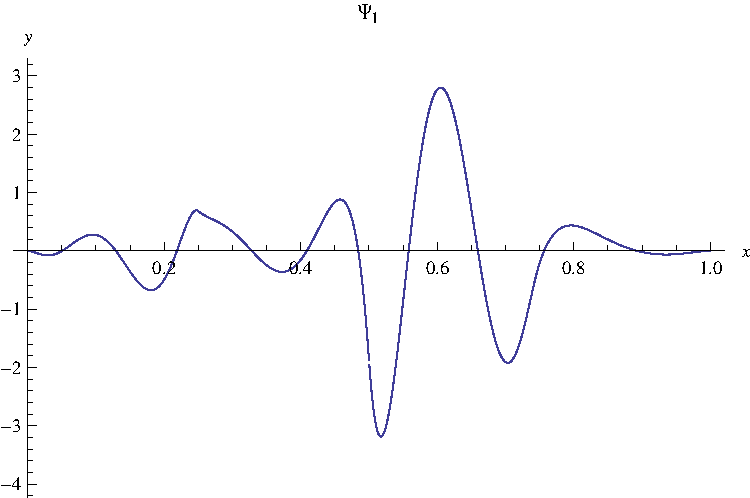
\includegraphics[width=5.0cm]{sextic_wavelet_1.pdf}& 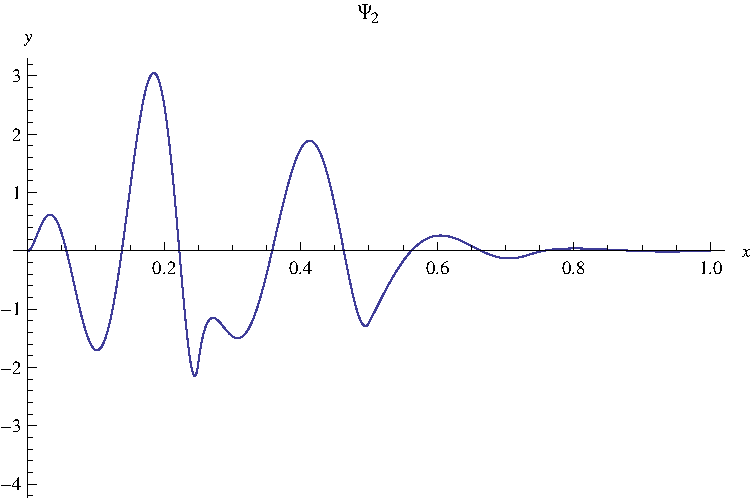
\includegraphics[width=5.0cm]{sextic_wavelet_2.pdf}& 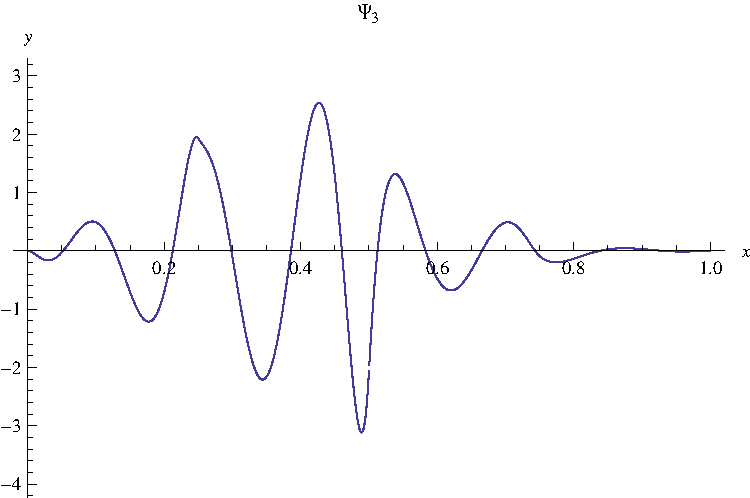
\includegraphics[width=5.0cm]{sextic_wavelet_3.pdf}& 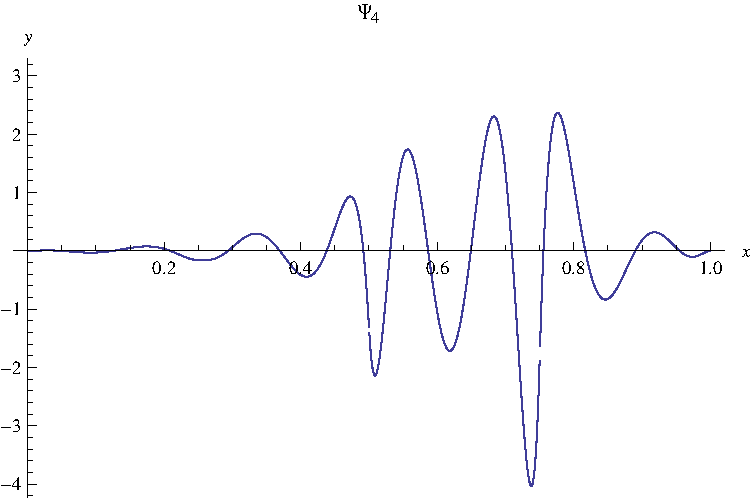
\includegraphics[width=5.0cm]{sextic_wavelet_4.pdf} \\
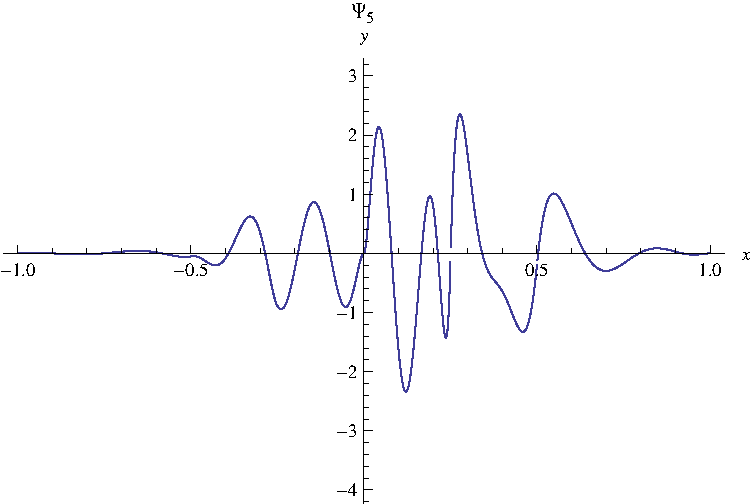
\includegraphics[width=5.0cm]{sextic_wavelet_5.pdf}& 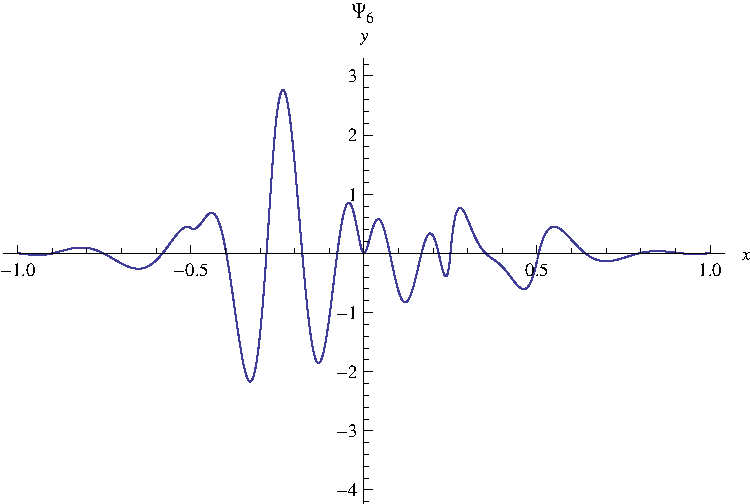
\includegraphics[width=5.0cm]{sextic_wavelet_6.pdf}& 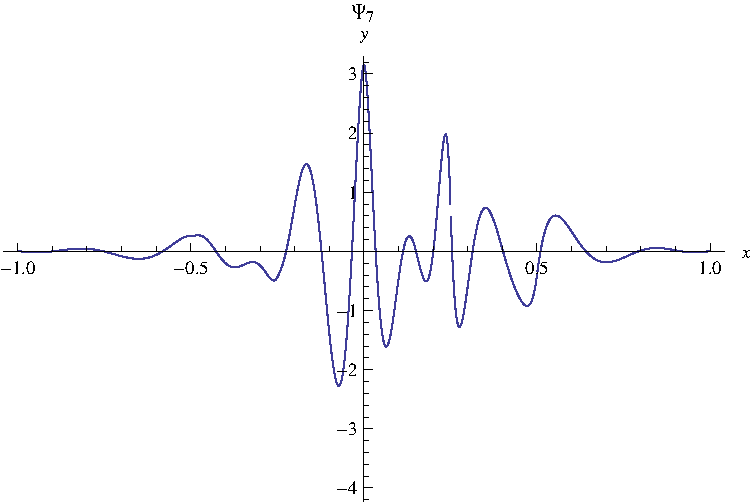
\includegraphics[width=5.0cm]{sextic_wavelet_7.pdf}& 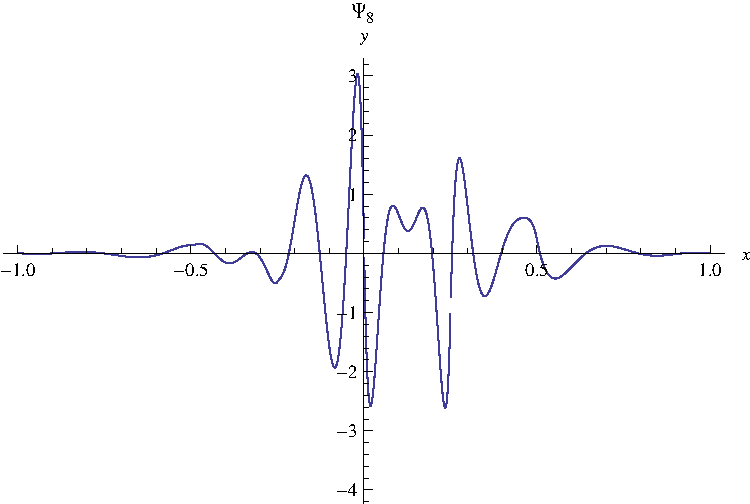
\includegraphics[width=5.0cm]{sextic_wavelet_8.pdf} \\
\end{tabular} 
 \end{landscape}
 \begin{landscape}
 \subsection{Validation}$$ \begin{array}{l|llllllll}
\int_{-1}^1 f_1(x)f_2(x) dx& \Psi_1(x)& \Psi_2(x)& \Psi_3(x)& \Psi_4(x)& \Psi_5(x)& \Psi_6(x)& \Psi_7(x)& \Psi_8(x) \\ \hline 
 \Psi_1(x) & 1.0000 & 0.\cdot 10^{(-206)} & 0.\cdot 10^{(-184)} & 0.\cdot 10^{(-115)} & 0.\cdot 10^{(-230)} & 0.\cdot 10^{(-230)} & 0.\cdot 10^{(-230)} & 0.\cdot 10^{(-230)} \\ 
\Psi_2(x) & 0.\cdot 10^{(-206)} & 1.0000 & 0.\cdot 10^{(-185)} & 0.\cdot 10^{(-116)} & 0.\cdot 10^{(-207)} & 0.\cdot 10^{(-207)} & 0.\cdot 10^{(-207)} & 0.\cdot 10^{(-207)} \\ 
\Psi_3(x) & 0.\cdot 10^{(-184)} & 0.\cdot 10^{(-185)} & 1.0000 & 0.\cdot 10^{(-115)} & 0.\cdot 10^{(-184)} & 0.\cdot 10^{(-185)} & 0.\cdot 10^{(-184)} & 0.\cdot 10^{(-184)} \\ 
\Psi_4(x) & 0.\cdot 10^{(-115)} & 0.\cdot 10^{(-116)} & 0.\cdot 10^{(-115)} & 1.0000 & 0.\cdot 10^{(-115)} & 0.\cdot 10^{(-116)} & 0.\cdot 10^{(-116)} & 0.\cdot 10^{(-116)} \\ 
\Psi_5(x) & 0.\cdot 10^{(-230)} & 0.\cdot 10^{(-207)} & 0.\cdot 10^{(-184)} & 0.\cdot 10^{(-115)} & 1.0000 & 0.\cdot 10^{(-341)} & 0.\cdot 10^{(-385)} & 0.\cdot 10^{(-385)} \\ 
\Psi_6(x) & 0.\cdot 10^{(-230)} & 0.\cdot 10^{(-207)} & 0.\cdot 10^{(-185)} & 0.\cdot 10^{(-116)} & 0.\cdot 10^{(-341)} & 1.0000 & 0.\cdot 10^{(-341)} & 0.\cdot 10^{(-341)} \\ 
\Psi_7(x) & 0.\cdot 10^{(-230)} & 0.\cdot 10^{(-207)} & 0.\cdot 10^{(-184)} & 0.\cdot 10^{(-116)} & 0.\cdot 10^{(-385)} & 0.\cdot 10^{(-341)} & 1.0000 & 0.\cdot 10^{(-646)} \\ 
\Psi_8(x) & 0.\cdot 10^{(-230)} & 0.\cdot 10^{(-207)} & 0.\cdot 10^{(-184)} & 0.\cdot 10^{(-116)} & 0.\cdot 10^{(-385)} & 0.\cdot 10^{(-341)} & 0.\cdot 10^{(-646)} & 1.0000 \\ 
\end{array} $$
$$ \begin{array}{l|llllllll}
\int_{-1}^1 f_1(x)f_2(x-1) dx& \Psi_1(x-1)& \Psi_2(x-1)& \Psi_3(x-1)& \Psi_4(x-1)& \Psi_5(x-1)& \Psi_6(x-1)& \Psi_7(x-1)& \Psi_8(x-1) \\ \hline 
 \Psi_1(x) & 0 & 0 & 0 & 0 & 0.\cdot 10^{(-228)} & 0.\cdot 10^{(-227)} & 0.\cdot 10^{(-227)} & 0.\cdot 10^{(-227)} \\ 
\Psi_2(x) & 0 & 0 & 0 & 0 & 0.\cdot 10^{(-205)} & 0.\cdot 10^{(-205)} & 0.\cdot 10^{(-205)} & 0.\cdot 10^{(-205)} \\ 
\Psi_3(x) & 0 & 0 & 0 & 0 & 0.\cdot 10^{(-183)} & 0.\cdot 10^{(-182)} & 0.\cdot 10^{(-182)} & 0.\cdot 10^{(-182)} \\ 
\Psi_4(x) & 0 & 0 & 0 & 0 & 0.\cdot 10^{(-114)} & 0.\cdot 10^{(-113)} & 0.\cdot 10^{(-113)} & 0.\cdot 10^{(-113)} \\ 
\Psi_5(x) & 0 & 0 & 0 & 0 & 0.\cdot 10^{(-383)} & 0.\cdot 10^{(-339)} & 0.\cdot 10^{(-383)} & 0.\cdot 10^{(-383)} \\ 
\Psi_6(x) & 0 & 0 & 0 & 0 & 0.\cdot 10^{(-340)} & 0.\cdot 10^{(-339)} & 0.\cdot 10^{(-339)} & 0.\cdot 10^{(-339)} \\ 
\Psi_7(x) & 0 & 0 & 0 & 0 & 0.\cdot 10^{(-383)} & 0.\cdot 10^{(-339)} & -5.65519\cdot 10^{(-463)} & -5.77195\cdot 10^{(-463)} \\ 
\Psi_8(x) & 0 & 0 & 0 & 0 & 0.\cdot 10^{(-384)} & 0.\cdot 10^{(-339)} & 5.01751\cdot 10^{(-463)} & 4.13609\cdot 10^{(-463)} \\ 
\end{array} $$ 
$$ \begin{array}{l|llllllll}
\int_{-1}^1 f_1(x)f_2(x) dx& \varphi_1(x)& \varphi_2(x)& \varphi_3(x)& \varphi_4(x)& \varphi_5(x)& \varphi_6(x)& \varphi_7(x)& \varphi_8(x) \\ \hline 
 \Psi_1(x) & 0.\cdot 10^{(-232)} & 0.\cdot 10^{(-232)} & 0.\cdot 10^{(-231)} & 0.\cdot 10^{(-230)} & 0.\cdot 10^{(-229)} & 0.\cdot 10^{(-230)} & 0.\cdot 10^{(-230)} & 0.\cdot 10^{(-229)} \\ 
\Psi_2(x) & 0.\cdot 10^{(-210)} & 0.\cdot 10^{(-210)} & 0.\cdot 10^{(-209)} & 0.\cdot 10^{(-208)} & 0.\cdot 10^{(-207)} & 0.\cdot 10^{(-207)} & 0.\cdot 10^{(-207)} & 0.\cdot 10^{(-207)} \\ 
\Psi_3(x) & 0.\cdot 10^{(-187)} & 0.\cdot 10^{(-187)} & 0.\cdot 10^{(-186)} & 0.\cdot 10^{(-185)} & 0.\cdot 10^{(-184)} & 0.\cdot 10^{(-184)} & 0.\cdot 10^{(-185)} & 0.\cdot 10^{(-184)} \\ 
\Psi_4(x) & 0.\cdot 10^{(-118)} & 0.\cdot 10^{(-118)} & 0.\cdot 10^{(-117)} & 0.\cdot 10^{(-116)} & 0.\cdot 10^{(-115)} & 0.\cdot 10^{(-115)} & 0.\cdot 10^{(-116)} & 0.\cdot 10^{(-115)} \\ 
\Psi_5(x) & 0.\cdot 10^{(-388)} & 0.\cdot 10^{(-388)} & 0.\cdot 10^{(-387)} & 0.\cdot 10^{(-386)} & 0.\cdot 10^{(-385)} & 0.\cdot 10^{(-386)} & 0.\cdot 10^{(-386)} & 0.\cdot 10^{(-386)} \\ 
\Psi_6(x) & 0.\cdot 10^{(-344)} & 0.\cdot 10^{(-344)} & 0.\cdot 10^{(-344)} & 0.\cdot 10^{(-342)} & 0.\cdot 10^{(-341)} & 0.\cdot 10^{(-342)} & 0.\cdot 10^{(-342)} & 0.\cdot 10^{(-341)} \\ 
\Psi_7(x) & -1.88585\cdot 10^{(-463)} & -4.2357\cdot 10^{(-464)} & -1.87128\cdot 10^{(-463)} & 1.82581\cdot 10^{(-463)} & 5.63403\cdot 10^{(-463)} & -3.11605\cdot 10^{(-464)} & 0.\cdot 10^{(-668)} & 0.\cdot 10^{(-668)} \\ 
\Psi_8(x) & 3.13585\cdot 10^{(-463)} & 5.36753\cdot 10^{(-464)} & 3.11163\cdot 10^{(-463)} & -2.07297\cdot 10^{(-463)} & -7.99791\cdot 10^{(-463)} & 8.22116\cdot 10^{(-464)} & 0.\cdot 10^{(-647)} & 0.\cdot 10^{(-647)} \\ 
\end{array} $$ 
$$ \begin{array}{l|llllllll}
\int_{-1}^1 f_1(x)f_2(x-1) dx& \varphi_1(x-1)& \varphi_2(x-1)& \varphi_3(x-1)& \varphi_4(x-1)& \varphi_5(x-1)& \varphi_6(x-1)& \varphi_7(x-1)& \varphi_8(x-1) \\ \hline 
 \Psi_1(x) & 0 & 0 & 0 & 0 & 0 & 0 & 0.\cdot 10^{(-230)} & 0.\cdot 10^{(-229)} \\ 
\Psi_2(x) & 0 & 0 & 0 & 0 & 0 & 0 & 0.\cdot 10^{(-207)} & 0.\cdot 10^{(-207)} \\ 
\Psi_3(x) & 0 & 0 & 0 & 0 & 0 & 0 & 0.\cdot 10^{(-185)} & 0.\cdot 10^{(-184)} \\ 
\Psi_4(x) & 0 & 0 & 0 & 0 & 0 & 0 & 0.\cdot 10^{(-116)} & 0.\cdot 10^{(-115)} \\ 
\Psi_5(x) & 0 & 0 & 0 & 0 & 0 & 0 & 0.\cdot 10^{(-386)} & 0.\cdot 10^{(-385)} \\ 
\Psi_6(x) & 0 & 0 & 0 & 0 & 0 & 0 & 0.\cdot 10^{(-342)} & 0.\cdot 10^{(-341)} \\ 
\Psi_7(x) & 0 & 0 & 0 & 0 & 0 & 0 & 4.21571\cdot 10^{(-463)} & 1.1142\cdot 10^{(-462)} \\ 
\Psi_8(x) & 0 & 0 & 0 & 0 & 0 & 0 & -4.00046\cdot 10^{(-463)} & -7.92331\cdot 10^{(-463)} \\ 
\end{array} $$ 
$$ \begin{array}{l|llllllll}
\int_{-1}^1 f_1(x)f_2(x+1) dx& \varphi_1(x+1)& \varphi_2(x+1)& \varphi_3(x+1)& \varphi_4(x+1)& \varphi_5(x+1)& \varphi_6(x+1)& \varphi_7(x+1)& \varphi_8(x+1) \\ \hline 
 \Psi_1(x) & 0 & 0 & 0 & 0 & 0 & 0 & 0 & 0 \\ 
\Psi_2(x) & 0 & 0 & 0 & 0 & 0 & 0 & 0 & 0 \\ 
\Psi_3(x) & 0 & 0 & 0 & 0 & 0 & 0 & 0 & 0 \\ 
\Psi_4(x) & 0 & 0 & 0 & 0 & 0 & 0 & 0 & 0 \\ 
\Psi_5(x) & 0.\cdot 10^{(-390)} & 0.\cdot 10^{(-389)} & 0.\cdot 10^{(-389)} & 0.\cdot 10^{(-386)} & 0.\cdot 10^{(-386)} & 0.\cdot 10^{(-387)} & 0.\cdot 10^{(-386)} & 0.\cdot 10^{(-386)} \\ 
\Psi_6(x) & 0.\cdot 10^{(-344)} & 0.\cdot 10^{(-344)} & 0.\cdot 10^{(-344)} & 0.\cdot 10^{(-341)} & 0.\cdot 10^{(-341)} & 0.\cdot 10^{(-342)} & 0.\cdot 10^{(-341)} & 0.\cdot 10^{(-341)} \\ 
\Psi_7(x) & -1.88585\cdot 10^{(-463)} & 3.64823\cdot 10^{(-464)} & -1.87128\cdot 10^{(-463)} & -2.70506\cdot 10^{(-463)} & -8.14069\cdot 10^{(-464)} & -1.74171\cdot 10^{(-463)} & 5.65412\cdot 10^{(-463)} & -1.18614\cdot 10^{(-462)} \\ 
\Psi_8(x) & -3.87696\cdot 10^{(-463)} & 5.82437\cdot 10^{(-464)} & -3.84702\cdot 10^{(-463)} & -4.59807\cdot 10^{(-463)} & -3.03029\cdot 10^{(-464)} & -3.27666\cdot 10^{(-463)} & 5.89166\cdot 10^{(-463)} & -1.02792\cdot 10^{(-462)} \\ 
\end{array} $$ 
\end{landscape} 
 \begin{landscape}
 \subsection{sextic Wavelet dirichlet boundary Functions}
 \begin{eqnarray*}
 \Psi_{\text{left},1} & = & \begin{array}{cc}
 \{ & 
\begin{array}{cc}
 -7.756894320603613910124329356128448349210\times 10^6 x^6+5.499665154781672478774349827343343804418\times 10^6 x^5-1.395663110033614110290002076807741080795\times 10^6 x^4+147187.3370082119984784157276141232326517 x^3-5113.149906750154961603127480407489510197 x^2-20.93891946633050045860698965493131828379 x & x\geq 0\land x<\frac{1}{4} \\
 1.419462336463702205153373861840245740797\times 10^6 x^6-3.470844020494158125163171447304300963410\times 10^6 x^5+3.495548113567348493625676905659811884252\times 10^6 x^4-1.855603892755150265046557869959907415773\times 10^6 x^3+547367.7290899402925464840420181912304750 x^2-85001.18177013903146810015849536911010870 x+5422.266315237275569388296327170177198461 & x\geq \frac{1}{4}\land x<\frac{1}{2} \\
 11657.08480833303534632329972380811150839 x^6-56609.13251694031562001331759847760684396 x^5+113326.5855575635195006960503358433069437 x^4-119596.9179284110481769729006571156986619 x^3+70100.40289254194320499064120603835562861 x^2-21613.24049540145385971999213456347787672 x+2735.217682314319604696219124467009301916 & \left(x\geq \frac{1}{2}\land x<\frac{3}{4}\right)\lor \left(x\geq \frac{3}{4}\land x<1\right)
\end{array}

\end{array}\\
\Psi_{\text{left},2} & = & \begin{array}{cc}
 \{ & 
\begin{array}{cc}
 -1.025387168255298476948410103033987132437\times 10^7 x^6+7.787303455474326459455856565114005479407\times 10^6 x^5-2.251626242898562445482233321936627752844\times 10^6 x^4+308231.6129642674628365257345405034605135 x^3-19785.84963850590465106993778074642380201 x^2+463.5832990730071965942914704788386435582 x & x\geq 0\land x<\frac{1}{4} \\
 2.278922132169857444460157441082308192914\times 10^6 x^6-5.505590356093980985501902780711261634364\times 10^6 x^5+5.494687794691102901281514863649011352081\times 10^6 x^4-2.896245939857038453084429546692977993891\times 10^6 x^3+849242.9177621974592660446681232901796915 x^2-131163.3930975860485125165601072037192533 x+8324.946188056184697254911827530528596924 & x\geq \frac{1}{4}\land x<\frac{1}{2} \\
 -7973.365607215615924681410496810692140123 x^6+38767.00648734646684812367329508146076999 x^5-77726.05047337078259146665717118228351364 x^4+82182.61231176391210828318979823436397970 x^3-48284.73698203009340977117805639369244404 x^2+14931.00012881294216802951190827027599436 x-1896.465865306829198517129277199432646239 & \left(x\geq \frac{1}{2}\land x<\frac{3}{4}\right)\lor \left(x\geq \frac{3}{4}\land x<1\right)
\end{array}

\end{array}\\ 
\Psi_{\text{right},1} & = & \begin{array}{cc}
 \{ & 
\begin{array}{cc}
 -5839.541382863514287664036175008748961358 x^6+7560.300820181297478572035478411000305963 x^5-3358.449749609645845720096136687399893104 x^4+585.8338036777386499472507714124721942282 x^3-31.96581889644324676780100619742345559438 x^2 & x\geq 0\land x<\frac{1}{2} \\
 -1.105986555469121298756140210659631719994\times 10^6 x^6+3.948470721197449726756971974332882284863\times 10^6 x^5-5.828177160013702442910271081734066724021\times 10^6 x^4+4.553503540677107261606683088051076715710\times 10^6 x^3-1.986505198115087661226196853707593267040\times 10^6 x^2+458937.3660464424247324919693641818536555 x-43877.57245853815895707632242974378233324 & x\geq \frac{1}{2}\land x<\frac{3}{4} \\
 2.813677875543937318249370256260315211251\times 10^6 x^6-1.444409282955747948037483410926099722842\times 10^7 x^5+3.078391050619402272318886730240532806445\times 10^7 x^4-3.486300627037017891566933646114416232516\times 10^7 x^3+2.212706066653284285578779679131300951088\times 10^7 x^2-7.462267214041950148373320521731858002750\times 10^6 x+1.044717265698805647191456742158364769758\times 10^6 & x\geq \frac{3}{4}\land x<1
\end{array}

\end{array}\\
\Psi_{\text{right},2} & = & \begin{array}{cc}
 \{ & 
\begin{array}{cc}
 3312.737593538316969911179618284889249844 x^6-4318.143004085687317188255202228400636020 x^5+1928.513250876287628196165596853458723675 x^4-337.8065587520413875106985789987714571876 x^3+18.49145777256589821005402863522875618707 x^2 & x\geq 0\land x<\frac{1}{2} \\
 -489987.1745746296413939716415079395886385 x^6+1.815284821022268872076975868803463696219\times 10^6 x^5-2.787740335453053285119507660432634951507\times 10^6 x^4+2.271245859539154291539337655997713863419\times 10^6 x^3-1.035294338226675076194805664708513545453\times 10^6 x^2+250327.3117362783711542831060287468125042 x-25083.88516346592400464413832041288697959 & x\geq \frac{1}{2}\land x<\frac{3}{4} \\
 5.426175040861877225437315859505543215353\times 10^6 x^6-2.758220742246096856910409826454711375269\times 10^7 x^5+5.826056541939043943647582732086937778794\times 10^7 x^4-6.545773191060748585381885199963096183927\times 10^7 x^3+4.126059400653951365673583398703691754345\times 10^7 x^2-1.383571793316666059627337969503983816118\times 10^7 x+1.928322799443284700547352791806075206402\times 10^6 & x\geq \frac{3}{4}\land x<1
\end{array}

\end{array}\end{eqnarray*}
\end{landscape}
\begin{landscape}
\subsection{Wavelet Dirichlet boundary Graphics}
\begin{tabular}{cc}
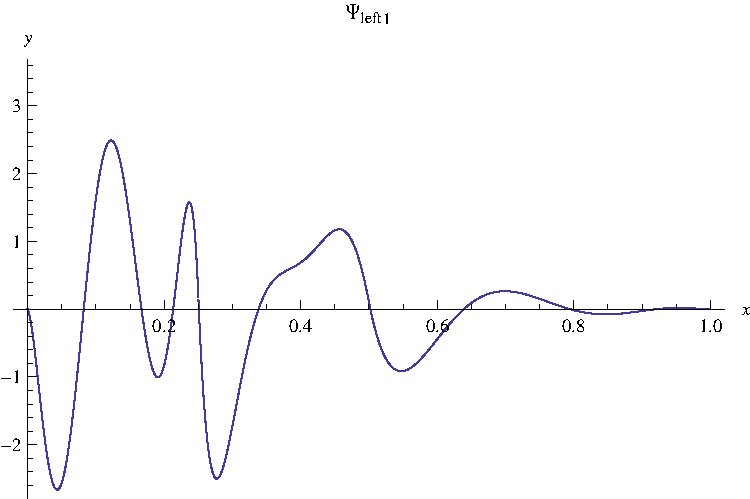
\includegraphics[width=10.cm]{sextic_wavelet_dleft_1.pdf}& 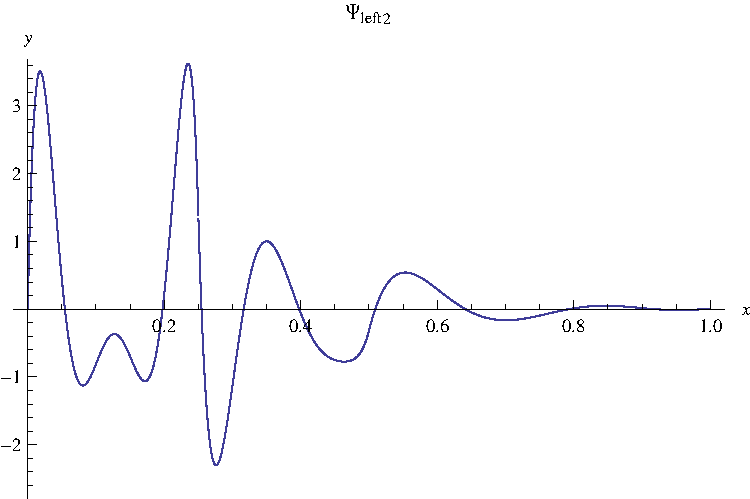
\includegraphics[width=10.cm]{sextic_wavelet_dleft_2.pdf} \\
\end{tabular} 
 \\ 
\begin{tabular}{cc}
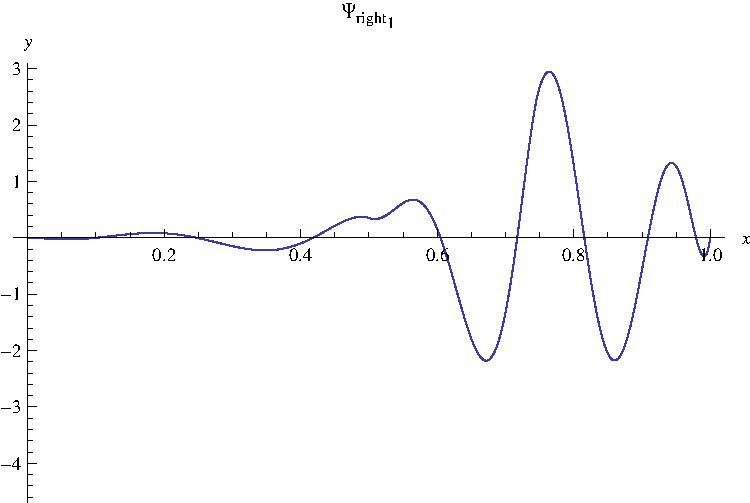
\includegraphics[width=10.cm]{sextic_wavelet_dright_1.pdf}& 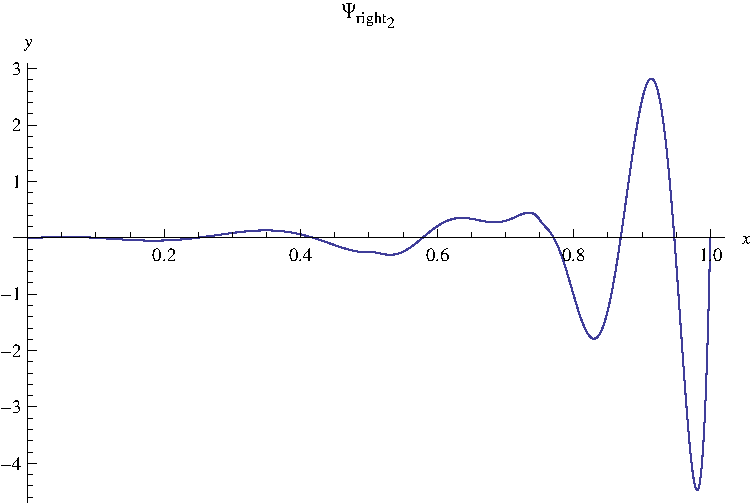
\includegraphics[width=10.cm]{sextic_wavelet_dright_2.pdf} \\
\end{tabular} 
 \end{landscape}
 \begin{landscape}
 \subsection{Validation}$$ \begin{array}{l|ll}
\int_{-1}^1 f_1(x)f_2(x) dx& \Psi_{\text{left},1}(x)& \Psi_{\text{left},2}(x) \\ \hline 
 \Psi_{\text{left},1}(x) & 1.0000 & 0.\cdot 10^{(-129)} \\ 
\Psi_{\text{left},2}(x) & 0.\cdot 10^{(-129)} & 1.0000 \\ 
\end{array} $$
$$ \begin{array}{l|llllllll}
\int_{-1}^1 f_1(x)f_2(x) dx& \varphi_1(x)& \varphi_2(x)& \varphi_3(x)& \varphi_4(x)& \varphi_5(x)& \varphi_6(x)& \varphi_7(x)& \varphi_8(x) \\ \hline 
 \Psi_{\text{left},1}(x) & 0.\cdot 10^{(-177)} & 0.\cdot 10^{(-176)} & 0.\cdot 10^{(-176)} & 0.\cdot 10^{(-174)} & 0.\cdot 10^{(-173)} & 0.\cdot 10^{(-174)} & -0.17062 & -0.010465 \\ 
\Psi_{\text{left},2}(x) & 0.\cdot 10^{(-132)} & 0.\cdot 10^{(-132)} & 0.\cdot 10^{(-131)} & 0.\cdot 10^{(-130)} & 0.\cdot 10^{(-129)} & 0.\cdot 10^{(-129)} & 0.21699 & 0.013310 \\ 
\end{array} $$ 
$$ \begin{array}{l|llllllll}
\int_{-1}^1 f_1(x)f_2(x) dx& \varphi_1(x-1)& \varphi_2(x-1)& \varphi_3(x-1)& \varphi_4(x-1)& \varphi_5(x-1)& \varphi_6(x-1)& \varphi_7(x-1)& \varphi_8(x-1) \\ \hline 
 \Psi_{\text{left},1}(x) & 0 & 0 & 0 & 0 & 0 & 0 & 0.\cdot 10^{(-174)} & 0.\cdot 10^{(-173)} \\ 
\Psi_{\text{left},2}(x) & 0 & 0 & 0 & 0 & 0 & 0 & 0.\cdot 10^{(-129)} & 0.\cdot 10^{(-129)} \\ 
\end{array} $$ 
$$ \begin{array}{l|llllllll}
\int_{-1}^1 f_1(x)f_2(x) dx& \Psi_1(x)& \Psi_2(x)& \Psi_3(x)& \Psi_4(x)& \Psi_5(x)& \Psi_6(x)& \Psi_7(x)& \Psi_8(x) \\ \hline 
 \Psi_{\text{left},1}(x) & 0.\cdot 10^{(-173)} & 0.\cdot 10^{(-174)} & 0.\cdot 10^{(-173)} & 0.\cdot 10^{(-116)} & -0.92320 & -0.31372 & 0.13555 & 0.038567 \\ 
\Psi_{\text{left},2}(x) & 0.\cdot 10^{(-128)} & 0.\cdot 10^{(-129)} & 0.\cdot 10^{(-128)} & 0.\cdot 10^{(-116)} & 0.\cdot 10^{(-129)} & 0.023126 & 0.56772 & -0.72994 \\ 
\end{array} $$ 
$$ \begin{array}{l|llllllll}
\int_{-1}^1 f_1(x)f_2(x) dx& \Psi_1(x-1)& \Psi_2(x-1)& \Psi_3(x-1)& \Psi_4(x-1)& \Psi_5(x-1)& \Psi_6(x-1)& \Psi_7(x-1)& \Psi_8(x-1) \\ \hline 
 \Psi_{\text{left},1}(x) & 0 & 0 & 0 & 0 & 0.\cdot 10^{(-172)} & 0.\cdot 10^{(-172)} & 0.\cdot 10^{(-172)} & 0.\cdot 10^{(-171)} \\ 
\Psi_{\text{left},2}(x) & 0 & 0 & 0 & 0 & 0.\cdot 10^{(-127)} & 0.\cdot 10^{(-127)} & 0.\cdot 10^{(-127)} & 0.\cdot 10^{(-127)} \\ 
\end{array} $$ 
$$ \begin{array}{l|l}
\int_{-1}^1 f_1(x)f_2(x) dx& \varphi_{\text{left},1}(x) \\ \hline 
 \Psi_{\text{left},1}(x) & 0.\cdot 10^{(-174)} \\ 
\Psi_{\text{left},2}(x) & 0.\cdot 10^{(-129)} \\ 
\end{array} $$ 
$$ \begin{array}{l|l}
\int_{-1}^1 f_1(x)f_2(x) dx& \varphi_{\text{right},1}(x) \\ \hline 
 \Psi_{\text{left},1}(x) & 0.\cdot 10^{(-173)} \\ 
\Psi_{\text{left},2}(x) & 0.\cdot 10^{(-129)} \\ 
\end{array} $$ 
$$ \begin{array}{l|ll}
\int_{-1}^1 f_1(x)f_2(x) dx& \Psi_{\text{right},1}(x)& \Psi_{\text{right},2}(x) \\ \hline 
 \Psi_{\text{right},1}(x) & 1.0000 & 0.\cdot 10^{(-210)} \\ 
\Psi_{\text{right},2}(x) & 0.\cdot 10^{(-210)} & 1.0000 \\ 
\end{array} $$
$$ \begin{array}{l|llllllll}
\int_{-1}^1 f_1(x)f_2(x) dx& \varphi_1(x)& \varphi_2(x)& \varphi_3(x)& \varphi_4(x)& \varphi_5(x)& \varphi_6(x)& \varphi_7(x)& \varphi_8(x) \\ \hline 
 \Psi_{\text{right},1}(x) & 0.\cdot 10^{(-276)} & 0.\cdot 10^{(-276)} & 0.\cdot 10^{(-275)} & 0.\cdot 10^{(-274)} & 0.\cdot 10^{(-273)} & 0.\cdot 10^{(-273)} & 0.\cdot 10^{(-274)} & 0.\cdot 10^{(-273)} \\ 
\Psi_{\text{right},2}(x) & 0.\cdot 10^{(-215)} & 0.\cdot 10^{(-215)} & 0.\cdot 10^{(-214)} & 0.\cdot 10^{(-213)} & 0.\cdot 10^{(-212)} & 0.\cdot 10^{(-212)} & 0.\cdot 10^{(-212)} & 0.\cdot 10^{(-212)} \\ 
\end{array} $$ 
$$ \begin{array}{l|llllllll}
\int_{-1}^1 f_1(x)f_2(x) dx& \varphi_1(x-1)& \varphi_2(x-1)& \varphi_3(x-1)& \varphi_4(x-1)& \varphi_5(x-1)& \varphi_6(x-1)& \varphi_7(x-1)& \varphi_8(x-1) \\ \hline 
 \Psi_{\text{right},1}(x) & 0 & 0 & 0 & 0 & 0 & 0 & 0.032026 & 0.0019644 \\ 
\Psi_{\text{right},2}(x) & 0 & 0 & 0 & 0 & 0 & 0 & -0.23957 & -0.014694 \\ 
\end{array} $$ 
$$ \begin{array}{l|llllllll}
\int_{-1}^1 f_1(x)f_2(x) dx& \Psi_1(x)& \Psi_2(x)& \Psi_3(x)& \Psi_4(x)& \Psi_5(x)& \Psi_6(x)& \Psi_7(x)& \Psi_8(x) \\ \hline 
 \Psi_{\text{left},1}(x) & 0.\cdot 10^{(-227)} & 0.\cdot 10^{(-205)} & 0.\cdot 10^{(-182)} & 0.\cdot 10^{(-113)} & 0.\cdot 10^{(-273)} & 0.\cdot 10^{(-274)} & 0.\cdot 10^{(-274)} & 0.\cdot 10^{(-274)} \\ 
\Psi_{\text{left},2}(x) & 0.\cdot 10^{(-211)} & 0.\cdot 10^{(-205)} & 0.\cdot 10^{(-182)} & 0.\cdot 10^{(-113)} & 0.\cdot 10^{(-212)} & 0.\cdot 10^{(-212)} & 0.\cdot 10^{(-212)} & 0.\cdot 10^{(-212)} \\ 
\end{array} $$ 
$$ \begin{array}{l|llllllll}
\int_{-1}^1 f_1(x)f_2(x) dx& \Psi_1(x-1)& \Psi_2(x-1)& \Psi_3(x-1)& \Psi_4(x-1)& \Psi_5(x-1)& \Psi_6(x-1)& \Psi_7(x-1)& \Psi_8(x-1) \\ \hline 
 \Psi_{\text{left},1}(x) & 0 & 0 & 0 & 0 & -0.34377 & 0.91932 & -0.15004 & -0.10109 \\ 
\Psi_{\text{left},2}(x) & 0 & 0 & 0 & 0 & 0.\cdot 10^{(-210)} & -0.17969 & -0.56505 & -0.67422 \\ 
\end{array} $$ 
$$ \begin{array}{l|l}
\int_{-1}^1 f_1(x)f_2(x) dx& \varphi_{\text{left},1}(x) \\ \hline 
 \Psi_{\text{right},1}(x) & 0.\cdot 10^{(-273)} \\ 
\Psi_{\text{right},2}(x) & 0.\cdot 10^{(-212)} \\ 
\end{array} $$ 
$$ \begin{array}{l|l}
\int_{-1}^1 f_1(x)f_2(x) dx& \varphi_{\text{right},1}(x) \\ \hline 
 \Psi_{\text{right},1}(x) & 0.\cdot 10^{(-273)} \\ 
\Psi_{\text{right},2}(x) & 0.\cdot 10^{(-212)} \\ 
\end{array} $$ 
$$ \begin{array}{l|ll}
\int_{-1}^1 f_1(x)f_2(x) dx& \Psi_{\text{left},1}(x)& \Psi_{\text{left},2}(x) \\ \hline 
 \Psi_{\text{right},1}(x) & 0.\cdot 10^{(-171)} & 0.\cdot 10^{(-127)} \\ 
\Psi_{\text{right},2}(x) & 0.\cdot 10^{(-171)} & 0.\cdot 10^{(-127)} \\ 
\end{array} $$ 
\end{landscape}
\end{document}

